\documentclass[11pt, aspectratio=169]{beamer}
% \documentclass[11pt,handout]{beamer}
\usepackage[T1]{fontenc}
\usepackage[utf8]{inputenc}
\usepackage{textcomp}
\usepackage{float, afterpage, rotating, graphicx}
\usepackage{epstopdf}
\usepackage{longtable, booktabs, tabularx}
\usepackage{fancyvrb, moreverb, relsize}
\usepackage{eurosym, calc}
\usepackage{amsmath, amssymb, amsfonts, amsthm, bm}
\usepackage[
    natbib=true,
    bibencoding=inputenc,
    bibstyle=authoryear-ibid,
    citestyle=authoryear-comp,
    maxcitenames=3,
    maxbibnames=10,
    useprefix=false,
    sortcites=true,
    backend=bibtex
]{biblatex}
\AtBeginDocument{\toggletrue{blx@useprefix}}
\AtBeginBibliography{\togglefalse{blx@useprefix}}
\setlength{\bibitemsep}{1.5ex}
\addbibresource{refs.bib}

\hypersetup{colorlinks=true, linkcolor=black, anchorcolor=black, citecolor=black, filecolor=black, menucolor=black, runcolor=black, urlcolor=black}

\setbeamertemplate{footline}[frame number]
\setbeamertemplate{navigation symbols}{}
\setbeamertemplate{frametitle}{\centering\vspace{1ex}\insertframetitle\par}

\DeclareMathOperator{\argmax}{arg\,max}

%Theorem
\newtheorem{assumption}{Assumption}
\newtheorem{proposition}{Proposition}
%\newtheorem{definition}{Definition}
%\newtheorem{theorem}{Theorem}


\begin{document}

\title{Topics in Behavioural Decision  Theory}

\author[Christian Hilpert]
{
{\bf Christian Hilpert}\\
{\small Lingnan College, Sun Yat-sen University}\\[1ex]
}


\begin{frame}
    \titlepage
    \note{~}
\end{frame}

\begin{frame}{Organisation}
    \begin{itemize}
        \item Contact: martin@mail.sysu.edu.cn\bigskip
        \item Office hours: Tuesday, 2:30 - 4:30 p.m., Office 301\bigskip
        \item Sign up here for a slot:
    \end{itemize}
    \centering
    \includegraphics[width = 0.2\textwidth]{OfficeHour}

\end{frame}

\begin{frame}{What are we doing}
    \begin{itemize}
        \item Overview of descriptive theories of choice under risk\bigskip
        \item Helps you think about behavioural aspects of finance/economics/insurance\bigskip
        \item Helps you to do research in this area\bigskip
    \end{itemize}
\end{frame}


\begin{frame}{Prerequisites}
    \begin{itemize}
        \item Microeconomics, in particular, decision theory\bigskip
        \item Applied mathematics - non-standard tools (Choquet integration)\bigskip
        \item Economic/financial intuition and interest in psychology\bigskip
    \end{itemize}
\end{frame}


\begin{frame}{Background}
    \begin{itemize}
        \item Who am I?\bigskip
        \item Who are you?\bigskip
        \item What are you interested in?\bigskip
        \item What do you expect from the course?\bigskip
    \end{itemize}
\end{frame}


\frame{\frametitle{Agenda}
\tableofcontents
}

\frame{\frametitle{Agenda}
\tableofcontents[currentsection]
}

%        \item Application and Limits of CPT\bigskip
   %     \item Alternative Theories\bigskip

\begin{frame}{Literature}
    \begin{itemize}
        \item \citet{Barberis2017Talk} AEA lecture: Behavioral Finance: Asset Prices and Investor Behavior\bigskip
        \item \citet{Malmendier2017Talk} AEA lecture: Behavioral Finance: Macro-finance, Experience Effects and Behavioral Corporate Finance\bigskip
        \item \citet{Thaler2016}:  Behavioral Economics: Past, Present, and Future.\bigskip
        \item \citet{Barberis2013a}: Thirty Years of Prospect Theory in Economics: A Review and Assessment\bigskip
        \item \citet{Wakker2010}, Prospect Theory for Risk and Ambiguity\bigskip
	\end{itemize}
\end{frame}

\section{Brief Overview of Behavioural Economics}
\begin{frame}{Brief overview}
    1950s-1990s: ''Traditional Finance''\bigskip
\begin{itemize}
	\item psychological shortcomings \bigskip
    \item new way of thinking about finance questions\bigskip
        \begin{enumerate}
            \item insurance\medskip
            \item portfolio choice\medskip
            \item corporate finance\ldots
            \medskip
        \end{enumerate}
    \item not alternative to mainstream economics (Micro)\bigskip
\end{itemize}
\end{frame}

\begin{frame}{Some questions}
    \begin{itemize}
        \item Why do people buy insurance, gamble, and hold stocks?\bigskip
        \item Why do people hold on to losing stocks?\bigskip
        \item Why are IPOs underpriced?\bigskip
    \end{itemize}
\end{frame}

\begin{frame}{Standard paradigm}
    \begin{itemize}
        \item $t= 0,1,2,...$ time\bigskip
        \item $S_t$ possible states\bigskip
        \item $p(s_t)$ probability of $s_t \in S_t$ occurring in $t$\bigskip
        \item $X_t$ payoff/consumption in $t$\bigskip
    \end{itemize}
\end{frame}

\begin{frame}{Standard paradigm}
\begin{itemize}
    \item Agent features utility function $U(X\mid S)$\medskip
    \begin{itemize}
\item time-independent discount factor $\delta $\medskip
\item implicitly: von-Neumann/Morgenstern axioms\medskip
\end{itemize}\bigskip

    \item Maximise expected lifetime utility\medskip
	\[\max_{x_t} \sum_t  \delta^t \left(\sum_{s_t \in S_t} U(x_t \mid s_t)\rho (s_t) \right) \qquad \text{s.t.} \quad x_t \in X_t\]
   \end{itemize}
\end{frame}


\begin{frame}{Behavioural decisions}
\begin{itemize}
\item Adjust optimisation:
	\[\max_{x_t} \sum_t  \delta^t \left(\sum_{s_t \in S_t} U(x_t \mid s_t)\rho (s_t) \right) \qquad \text{s.t.} \quad x_t \in X_t\]\bigskip
        \item Non-standard preferences: $U$, $\delta $\bigskip
        \item Non-standard beliefs: $\rho$\bigskip
        \item Non-standard decision making: $\max$\bigskip
\end{itemize}
\end{frame}


\begin{frame}{Alternative theories of choice under risk}
    \begin{enumerate}
        \item Reference-dependence, prospect theory, ambiguity\medskip
        \begin{itemize}
        \item Implies: loss aversion, non-standard time preferences, self-control issues, time inconsistency, social preferences
        \end{itemize}\medskip
        \item Overconfidence, extrapolation, experience effects\medskip
         \begin{itemize}
        \item Implies: overestimation, confirmation bias, projection bias, law of small numbers.  \end{itemize}\medskip
                \item Bounded rationality, cognitive limitations.\medskip
        \begin{itemize}
        \item Implies: rules of thumb, simplification, framing
        \end{itemize}\medskip
    \end{enumerate}
    Not sharply separated.  1 weakest, 3 strongest departure  from EU
\end{frame}

\begin{frame}{Alternatives}
    \begin{itemize}
        \item Bounded rationality\bigskip
        \item Evolutionary game theory\bigskip
        \item Decision theory (unawareness, unforeseen contingencies)\bigskip
    \end{itemize}\bigskip
\end{frame}
\begin{frame}{Behavioural economics is controversial!}
    \begin{itemize}
        \item Poor experimental standards\medskip
        \item Departure from revealed preference approaches\medskip
        \item Anything goes\medskip
    \end{itemize}
\end{frame}

\section{Cumulative Prospect Theory}
\frame{\frametitle{Agenda}
\tableofcontents[currentsection]
}
\begin{frame}{Prospect Theory and Cumulative Prospect Theory}
    \begin{itemize}
        \item Most finance models assume expected utility theory to evaluate risks\bigskip
        \item Experimentally, at least, not a good fit\bigskip
        \item \citet{KahnemanTversky1979}: prospect theory\bigskip
        \item \citet{TverskyKahneman1992}: cumulative prospect theory\bigskip
        \item Alternatives: disappointment aversion, rank-dependent utility, salience theory, regret theory, SP\&A theory\bigskip
    \end{itemize}
\end{frame}


\begin{frame}{Prospect Theory and Cumulative Prospect Theory}
    \begin{itemize}
        \item A reference-dependent utility function is a family $\{U(\cdot \mid \gamma):x \longrightarrow \mathbb{R} \mid \gamma \in X\}$  of utility functions over $X$ indexed by $\gamma \in X$.\bigskip
        \item The utility $U(X \mid \gamma)$ describes consumption utility while the reference point is $\gamma$.\bigskip
        \item Prospect theory vs expected utility theory: Consider gamble $L = (x, p, y, q)$\bigskip
        \item $EU = p V(w + x) + q V(w + y)$\bigskip
        \item $PT = w(p) V(x) + w(q) V(y)$\bigskip
\end{itemize}
\end{frame}


\begin{frame}{Expected utility}
    \begin{figure}
\centering
\includegraphics[width= 0.75\textwidth]{expected_utility}
\caption{Own computation with $\gamma =0.5$.}
    \end{figure}
\end{frame}

\begin{frame}{Cumulative prospect theory value function}
    \begin{figure}
\centering
\includegraphics[width= 0.75\textwidth]{cpt_utility}
\caption{\citet{Barberis2012a}, Figure 1a with $\lambda = 2.5$ and $\gamma =0.5$.}
    \end{figure}
\end{frame}


\begin{frame}{Four key features}
    \begin{enumerate}[1.]
        \item Reference-dependence:\medskip
            \begin{itemize}
                \item Gains and losses instead of final wealth.\medskip
                \item Experimental evidence consistent with perception of alternative.\medskip
            \end{itemize}\bigskip
        \item Loss aversion:\medskip
            \begin{itemize}
                \item $V(x)$ has a kink in zero.\medskip
                \item Losses loom larger than gains.\medskip
                \item Evidence: $(110,\frac{1}{2},-100,\frac{1}{2})$ is unattractive.
            \end{itemize}
    \end{enumerate}
\end{frame}

\begin{frame}{Four key features}
    \begin{enumerate}[3.]
        \item Diminishing sensitivity:\medskip
            \begin{itemize}
                \item $V(\cdot)$ is concave over gains, convex over losses. Evidence:
               \[(500,1) \succ \left(1000,\frac{1}{2}\right) \qquad \text{and}
                \qquad (-500,1) \preceq  \left(-1000,\frac{1}{2}\right).\]
            \end{itemize}
    \end{enumerate}
\end{frame}

\begin{frame}{Four key features}
    \begin{enumerate}[4.]
        \item Probability weighting:\medskip
            \begin{itemize}
                \item Transform probability with decision weights $w(\cdot)$:
                high weight on low probabilities.\medskip
                \item Evidence: Lotteries are attractive: \[(5,1)\prec (5000,0.001).\]
                \item Evidence: Insurance is attractive: \[(-5,1)\succ (-5000,0.001).\]
            \item Note: $w$ are decision weights not beliefs.
        \end{itemize}
    \end{enumerate}
\end{frame}



\begin{frame}{Cumulative Prospect Theory (Tversky and Kahneman, 1992)}
    \begin{itemize}
        \item \citet{TverskyKahneman1992} address some limitations (FOSD) of the original \citet{KahnemanTversky1979} prospect theory.\bigskip
        \item They apply probability weighing to the cumulative distribution function.\bigskip
        \item Example: gain at least 50, lose 100 or more.\bigskip
        \item Formally, consider
        \[(x_{-m},p_{-m},...,x_{-1},p_{-1},x_0,p_0,x_1,p_1,...,x_n,p_n)\]
        with $x_i < x_j$ for $i<j,x_0=0$.\bigskip
         \end{itemize}
\end{frame}

\begin{frame}{Cumulative Prospect Theory (Tversky and Kahneman, 1992)}
    \begin{itemize}
       \item The value assigned equals
        \[ \sum_{i=-m}^{n} \pi_i V(x_i)\]
        with
            \begin{equation}
                \pi_i = \begin{cases}
                w(p_i+...+p_n) - w(p_i+...+p_n),  & 0\leq i \leq  n\\
                w(p_{-m}+...+p_i) - w(p_{-m}+...+p_{i-1}),  & -m\leq i \leq 0\\
            \end{cases}
            \end{equation}\medskip
        \item Individuals overweight fails of a probability distribution.\medskip
        \item Preserves a taste for lottery like gambles.\medskip
    \end{itemize}
\end{frame}

\begin{frame}{Cumulative prospect theory decision weights}
    \begin{figure}
\centering
\includegraphics[width= 0.65\textwidth]{cpt_weights}
\caption{\citet{Barberis2012a}, Figure 1b with $\delta = 1$ (yellow), $\delta =0.65$ (blue), and $\delta =0.4$ (red).}
    \end{figure}
\end{frame}

\begin{frame}{Cumulative Prospect Theory (Tversky and Kahneman, 1992)}
    \begin{itemize}
        \item \citet{TverskyKahneman1992} suggest:
\begin{equation}
    V(x) = \begin{cases}
    x^\alpha,  & x\geq 0\\
    -\lambda (-x)^\alpha,  & x< 0\\
    \end{cases}
\end{equation}\medskip
\item with \[w(p) = \frac{p^{\delta}}{(p^{\delta}+(1-p)^{\delta})^{\frac{1}{\delta}}}\]
\item Their (questionable) estimates are $\alpha =0.88$, $\lambda =2.25$, and  $\delta =0.69$\medskip
    \item There are alternatives to formalise $w$.
\end{itemize}
\end{frame}

\begin{frame}{Challenges and discussion - value function}
    \begin{itemize}
        \item How to define gains and losses?\bigskip
        \item Total wealth, financial wealth, stock holdings, individual stocks?\bigskip
        \item What is a gain:\medskip
        \begin{itemize}
            \item exceeds zero?\medskip
            \item risk-free rate?\medskip
            \item expectation?\medskip
        \end{itemize}
                \item Diminishing sensitivity: \citet{Rabin2000}'s critique (not important feature theoretically)\medskip
        \end{itemize}
        \end{frame}

      \begin{frame}{Challenges and discussion - decision weights}
    \begin{itemize}
        \item Probability weighting in many applications more important than loss aversion.\medskip
        \item Overweighting vs underweighting: black swan events: \citet{Taleb2010}.\medskip
        \item There is evidence for both cases.\medskip
        \item Could be either \medskip
        \begin{itemize}
        \item Decision from description $\Rightarrow$ overweighting.\smallskip
        \item Decision from experience $\Rightarrow$ underweighting.\smallskip
        \end{itemize}
    \end{itemize}
\end{frame}


\begin{frame}{Challenges and discussion - decision weights}
    \begin{itemize}
        \item Not clear how to interpret:\medskip
          \begin{itemize}
        \item overestimation (belief) $\Rightarrow$ mistake.\smallskip
        \item overweighting (preference) $\Rightarrow$ not mistake.\smallskip
       \item There is some evidence pointing towards preferences.\medskip
           \end{itemize}
    \end{itemize}
\end{frame}

\section{Applications and Limitations of Cumulative Prospect Theory}

\frame{\frametitle{Agenda}
\tableofcontents[currentsection]
}


\begin{frame}{Applications and Limitations of CPT}
    Three sample applications to highlight:\bigskip
        \begin{enumerate}[i)]
            \item How to apply CPT\bigskip
            \item Interesting applications on their own\bigskip
            \item Key limitations of CPT\bigskip
        \end{enumerate}
    \end{frame}

\frame{\frametitle{Agenda}
\tableofcontents[currentsubsection]
}


\subsection{Monopolistic insurance and probability weighting}
    \begin{frame}{CPT customers in monopolistic markets - Setup}
        \begin{itemize}
            \item \citet{AzevedoGottlieb2012} ask what happens in strategic and market environments with CPT customers?\bigskip
            \item They consider a monopolistic insurer and CPT customers.\bigskip
                \item Monopolist can charge any arbitrarily large price policy features unbounded gains or losses with probability approaching zero.\bigskip
                \item Counterintuitive: insurance raises risk; no solution to firm's problem.\medskip
        \end{itemize}
    \end{frame}

    \begin{frame}{CPT customers in monopolistic markets - Preview}
        \begin{itemize}
            \item \citet{AzevedoGottlieb2012} show that for any insurance policy, there is always another policy that makes both the firm and consumers simultaneously better off.\bigskip
            \item If consumer's wealth is bounded, the insurer can extract all wealth with probability approaching one.\bigskip
            \item With Bertrand competition, no equilibrium exists.\bigskip
        \end{itemize}
    \end{frame}



    \begin{frame}{CPT customers in monopolistic markets - Preview}
        Additionally,\medskip
           \begin{itemize}
               \item Either, individuals pay arbitrarily large amounts for lotteries with finite expected value.\bigskip
               \item Or, individuals refuse all actuarially fair gambles.\bigskip
               \item First case implies no equilibrium if supply is endogenous.\bigskip
               \item Second case rules out simultaneous risk-seeking and aversion (why we use CPT in the first place).\bigskip
           \end{itemize}
       \end{frame}

       \begin{frame}{Model of monopolistic insurance and CPT customers}
           \begin{itemize}
               \item Gamble: $\mathcal{L} =(g, p; L, 1 - p), g \geq 0, -L\leq 0 $\medskip
               \item CPT  customer has preferences:\medskip
               \begin{itemize}
                \item $V(\mathcal{L} )= w^{+}(p)v(g)-\lambda w^{-}(1-p)v(L).$\medskip
                \item $w^{+},w^{-}:[0,1] \longrightarrow [0,1]$,\quad $ v:\mathbb{R}_{+} \longrightarrow \mathbb{R}$\medskip
               \end{itemize}\medskip
               \item Assumptions:\medskip
               \begin{itemize}
                \item $v$ is continuous, strictly increasing, $v(0)=0$,\medskip
                \item $ w^{+},w^{-}$ are continuous, strictly increasing\medskip
                \item $w^{+}(0)=w^{-}(0)=0$; $w^{+}(1)=w^{-}(1)=1$\medskip
               \end{itemize}
           \end{itemize}
       \end{frame}

       \begin{frame}{Model of monopolistic insurance and CPT customers}
        \begin{itemize}
            \item Risk-neutral firm designs $\mathcal{L}$, perfect information, monopolist.\bigskip
            \item Monopolist's profit: \[\pi(\mathcal{L})=(1-p)L-pg\]\bigskip
            \item Monopolist maximises expected profit s.t. $V(\mathcal{L})\geq 0$ (participation constraint)\bigskip
        \end{itemize}
    \end{frame}

       \begin{frame}{Key result of CPT under monopolistic insurance}
           \begin{proposition}
           Suppose either:\medskip
           \begin{enumerate}[(1)]
               \item $\lim_{p \to 0} w^{+}(p)v\left(\frac{1}{p}\right)=\infty$, or\medskip
               \item $\lim_{p \to 0} w^{-}(p)v\left(\frac{1}{p}\right)=0$\medskip
           \end{enumerate}
           Then, for any $K_1,K_2$, there exists a lottery $\mathcal{L}$
           s.t. $\pi(\mathcal{L}) \geq K_1$ and $V(\mathcal{L}) >v(K_2)$.
           In particular, $\Pi(V)=\infty.$
           \end{proposition}
           \hspace*{\fill} \\
       \textbf{Proof:} Blackboard.
    %    \begin{itemize}
    %        \item Consider the lottery$ (\frac{1}{p},p;\frac{1+\pi}{1-p},1-p)$.\\
    %        \item Assume (1) $\Rightarrow \mathbb{E} [\cdot]= (1- p)\frac{1+\pi}{1-p}-\frac{1}{p}p =\pi  $\\
    %    and $\lim_{p \to 0} w^{+}(p)v(\frac{1}{p})- \lambda w^{-}(1-p)v(\frac{1+\pi}{1-p})  $
    %    $\geq \lim_{p \to 0} w^{+}(p)v(\frac{1}{p})- \lambda v(1+\pi)$\\
    %    $\Rightarrow $  arbitrarily high utility, profit $\pi >0$.
    %    \end{itemize}
       \end{frame}



    %    \begin{frame}
    %        \begin{itemize}
    %            \item Assume (2). Consider:$ (\frac{u}{p},p;\frac{\pi+u}{1-p},1-p), u,\pi \geq 0.$\\
    %        $ \mathbb{E} [\cdot]= (1- p)\frac{\pi+u}{1-p}-\frac{u}{p}p =\pi  $\\
    %        \item CPT:$ w^{+}(p)v(\frac{u}{p})- \lambda w^{-}(1-p)v(\frac{u+\pi}{1-p})  $\\
    %        \item the limit:\\
    %     $\lim_{p \to 1}w^{+}(p)v(\frac{u}{p})- \lambda w^{-}(1-p)v(\frac{u+\pi}{1-p})$\\
    %        $=v(u) -\lambda \lim_{p \to 0} w^{-}(p)v(\frac{\pi+u}{p})=v(u)$\\
    %        \item $\Rightarrow $  any profit $\pi \geq 0$ ,any utility $v(u) \in [0,v(\infty))$,$p$ close to $1$.
    %    \end{itemize}
    %    \end{frame}

       \begin{frame}{Interpretation: Condition 1 - Lottery}
       \begin{itemize}
                \item Large sum $\frac{1}{p}$ with low $p$, and $0$ else.\bigskip
               \item Expected value is one, gain $\frac{1}{p}$ grows unboundedly as $p \rightarrow 0$.\bigskip
               \item Customer pays arbitrary amounts for expected value of 1.\bigskip
               \item Implies infinite expected firm profits, gives arbitrarily large certainty equivalents.\bigskip
           \end{itemize}
        \end{frame}

        \begin{frame}{Interpretation: Condition 2 - Insurance}
            \begin{itemize}
           \item Large loss $\frac{1}{p}$, with low probability $p$ implies an expected payment $=-1$ and unbounded loss $\frac{1}{p}$\medskip
               \item Implies arbitrarily small risk premium.\medskip
               \item Customer accepts negative expected payoff for arbitrarily small prices, firm again has infinite profits, customer infinite utility.\medskip
               \item Catastrophe bonds below fair price.\medskip
               \item Under both conditions, the firm has infinite profits for any lottery. There always is a better one for \alert{both} firm and customers as $p \rightarrow 0$.\medskip
       \end{itemize}
       \end{frame}

       \begin{frame}{Additional results - homogenous value function}
           \begin{itemize}
               \item Additionally, suppose $v(x)=x^\alpha, 0<\alpha \leq 1$, that is, homogeneous of degree $\alpha$.\bigskip
               \item For any two lotteries $\mathcal{L} =(g,p;L,1-p) $ and
               $c\mathcal{L} =(cg ,p; c L,1 - p)$, it holds that \[V(c\mathcal{L}) = c^\alpha V(\mathcal{L}), c>0  \Rightarrow  v(c\mathcal{L}) \geq  V(\mathcal{L})\].
               \item If individual accepts $\mathcal{L}$, he must also accept $c\mathcal{L}$, hence firm profits $\pi \rightarrow c\pi.$\bigskip
               \item If a seller can obtain a positive profit, it can obtain any positive profit.\bigskip
           \end{itemize}
       \end{frame}

       \begin{frame}{Some remarks}
           \begin{itemize}
               \item The choice of $\omega$ empirically does not matter.\bigskip
               \item All estimated forms of $\omega$ satisfy our conditions.\bigskip
               \item Adding a reference point $r\neq 0$ does not change anything.\bigskip
           \end{itemize}
       \end{frame}

       \begin{frame}{Some remarks}
        \begin{itemize}
            \item Competition $\grave{a}~la$ Bertrand destroys all equilibria.\bigskip
            \item Heterogeneity and private information do not matter for result.\bigskip
            \item Wealth constraints $B>0$ bounds profits, remaining analysis remains\bigskip
            \item Possible solution: global + local utility (next lecture)\bigskip
        \end{itemize}
    \end{frame}


\subsection{Casino gambling and time inconsistency}
\frame{\frametitle{Agenda}
\tableofcontents[currentsubsection]
}

\begin{frame}{Casino gambling and CPT}
    \begin{itemize}
        \item Consider \citet{Barberis2012a}'s model of casino gambling of a CPT agent.\bigskip
        \item Why do people gamble?\bigskip
        \item Why can CPT shed light on this matter? Loss aversion?\bigskip
        \item Even probabilities are unappealing because of probability weighting (not skew!)\bigskip
        \item General take-away: Timing and time-inconsistency.\bigskip
    \end{itemize}
\end{frame}

\begin{frame}{Casino gambling and CPT}
    \begin{itemize}
        \item \citet{Barberis2012a} shows that CPT agents gamble for many parameters despite zero skewness and negative or zero outcomes.\medskip
        \item CPT implies time-inconsistent behaviour.\medskip
        \item Consider a series of $50/50$ bets. Isolated bet is unattractive.\medskip
        \item Initial plan: play if winning, quit on losing.\medskip
        \item Composite bet is attractive! Low loss, high upside!\medskip
        \item Play five times. Ex-ante: $P(win\, 5 \times) = 1/32$.\medskip
        \item Probability weighting implies overweighting.\medskip
    \end{itemize}
\end{frame}

\begin{frame}{Casino gambling and CPT}
    \begin{itemize}
        \item After playing four times: $P(win\, 5 \times) = 1/2$. Underweighted!\bigskip
        \item Preference changes over time.\bigskip
        \item CPT predicts heterogeneity in gambling behavior:\bigskip
        \begin{enumerate}
            \item Naive agent: plans, deviates from plan.\medskip
            \item Sophisticated agent: knows time inconsistency, cannot commit
            $\Rightarrow$ predicts losing.\medskip
            \item Sophisticated agent with commitment $\Rightarrow$ predicts behaviours, sticks with (eg: only takes limited cash).\medskip
        \end{enumerate}
    \end{itemize}
\end{frame}


\begin{frame}{A model of casino gambling based on roulette}
    \begin{itemize}
    \item Same as before:\medskip
        \[
        v(x) = \begin{cases}
            x^\alpha  &  \text{for} \quad x \geq 0,\\
            -\lambda (-x)^\alpha & \text{for} \quad x<0,
            \end{cases}
        \]\medskip
        and \\
        {\centering $ \omega(p)=\frac{p^\delta }{(p^\delta + (1-p)^\delta)^{\frac{1}{\delta}}} $\\

        }
        \hspace*{\fill} \\
    \item General parameter space  with $\alpha \in (0,1], \lambda>1,  \delta \in (0,1 $ with $T+1$ dates, $t=0,1,...,T.$ \medskip
    \item At $t=0$, $50:50$ bet: gain/lose $h$. At any time bet, if declines once, game is over.\medskip
    \end{itemize}
\end{frame}

\begin{frame}{Binomial tree representation of casino, 5 periods}
    \begin{figure}
\centering
        \includegraphics[width = 0.35\textwidth]{fig2.png}
    \caption{\citet{Barberis2012a}, Figure 2. Black: no gamble; white: gamble}
    \end{figure}
    \end{frame}

\begin{frame}{Binomial Tree Representation}
    \begin{itemize}
        \item Represent each node as $(t, j)$.\bigskip
        \item Time $t \in {0,\ldots ,T}$ \bigskip
        \item Wealth $ j \in {1,\ldots, t+1}$, counts how far down. $j=1$ represents the top node.\bigskip
        \item Assume: reference point is $r=0$. Compute the CPT value of the whole evening.\bigskip
    \end{itemize}
\end{frame}


\begin{frame}{Time inconsistency}
    \begin{itemize}
        \item Time inconsistency: Consider node $(4,1)$.\medskip
        \item Initial probability $\frac{1}{32}$: gain 50 or down 30  $\Rightarrow$ gamble. If actually at node $(4,1)$:
        \begin{align*}v(40) &\geq v(50)\omega \left(\frac{1}{2}\right)+v(30)\left(1-\omega \left(\frac{1}{2}\right)\right) \Rightarrow \text{ usually exit.}\\
        \Leftrightarrow v(40)-v(30) &\geq (v(50)-v(30))\omega \left(\frac{1}{2}\right)\end{align*}
        \item Holds for all $\alpha, \delta \in (0,1)$.\medskip
        \item Similar: initial plan: stop at (4,5), stop gambling.\medskip
    \end{itemize}
\end{frame}


\begin{frame}{Gambling strategies and CPT values}
    \begin{itemize}
        \item General description for fixed strategies $s \in S(0,1)$.\bigskip
        \item Example: coloured strategy $\tilde{g_s}$:\bigskip
        \item $\tilde{g_s} \backsim \left(30,\frac{7}{32}; 10,\frac{9}{32}; -10, \frac{10}{32}; -30,\frac{5}{32};-50,\frac{1}{32} \right)  $\bigskip
        \item Maximise the expected value of the strategy: $\max_{s \in S(0,1)} V(\tilde{g_s})$\bigskip
        \item Generally no analytically solution.\bigskip
    \end{itemize}
\end{frame}

\begin{frame}{Numerical analysis - Naive agent}
    \begin{itemize}
        \item Many parameters enter, that is, $V(\tilde{g_s})>0 $\medskip
        \item Deviations for naive agent: $(\alpha,\delta,\lambda)=(0.95,0.5,1.5)$ in the following\medskip
    \end{itemize}
\end{frame}

\begin{frame}{Naive agent - plan}
\begin{figure}
\centering
    \includegraphics[width = 0.35\textwidth]{naive_plan.png}
    \caption{\citet{Barberis2012a}, Figure 4a.}
    \end{figure}
\end{frame}

\begin{frame}{Naive agent - actual}
\begin{figure}
\centering
    \includegraphics[width = 0.35\textwidth]{naive_final.png}
    \caption{\citet{Barberis2012a}, Figure 4b.}
    \end{figure}
\end{frame}


\begin{frame}{Naive vs sophisticated agent}
    \begin{itemize}
    	\item \textbf{Naive agent}:\medskip
        \item Mostly: plan a "loss exit" strategy, some: plan a "gain exit" strategy.\medskip
        \item Probability weighting mostly  dominates loss aversion.\bigskip
  	    \end{itemize}
\end{frame}

\begin{frame}{Naive agent - participation}
\begin{figure}
\centering
    \includegraphics[width = 0.45\textwidth]{cpt_naive}
    \caption{\citet{Barberis2012a}, Figure 3. $\star$ represents staying if winning. $+$ represents staying if losing.}
    \end{figure}
\end{frame}

\begin{frame}{Naive vs sophisticated agent}
    \begin{itemize}
     	\item \textbf{Sophisticated without commitment}:\medskip
        \item Aware of time inconsistency, uses backward induction\medskip
        \item At node $(t, j), t \in [0,T-1]$:\medskip
        \begin{itemize}
        \item If the value of continuing to gamble $V(\tilde{g_{t,j}}) > v(h(t+2-2j))$ exceeds value of leaving immediately, gamble\medskip
        \item Agent rarely enters casino; only if  $\alpha,\lambda $ small,$\delta$ large\medskip
        \end{itemize}
    \end{itemize}
\end{frame}

\begin{frame}{Sophisticated agent without commitment - participation}
\begin{figure}
\centering
    \includegraphics[width = 0.45\textwidth]{cpt_sophisticated}
    \caption{\citet{Barberis2012a}, Figure 5. $\star$ represents staying if winning. $+$ represents staying if losing.}    \end{figure}
\end{frame}


\begin{frame}{Sophisticated agent with commitment}
    \begin{itemize}
        \item Same as naive agent, but goes through with plans.\medskip
        \item No time inconsistency.\medskip
        \item Eliminates gambling in the region of losses.\medskip
        \item Reality: takes a small amount of cash.\medskip
    \end{itemize}
\end{frame}


\subsection{Skewness preference in the small}
\frame{\frametitle{Agenda}
\tableofcontents[currentsubsection]
}


\begin{frame}{Dynamic approach to gambling under CPT}
    \begin{itemize}
        \item Consider \citet{EbertStrack2015}.\medskip
        \item Take a dynamic perspective on gambling decisions under CPT.\medskip
        \item Key takeaway: CPT agent never stops gambling/investing.\medskip
        \item Key property: "Skewness preference in the small".\medskip
        \item Opposite of \citet{AzevedoGottlieb2012} - huge gambles.\medskip
	\end{itemize}
\end{frame}

\begin{frame}{Skewness preference in the small}
    \begin{itemize}
        \item Consider a simple, small, lottery-like risk with negative expectation.\medskip
        \item Idea of the CPT gambler: If I lose a bit more, I stop.\medskip
        \item Investment: never exercise attractive  options\medskip
        \item Key assumption: probability weighting dominate loss aversion\medskip
	\end{itemize}
\end{frame}

\begin{frame}{Model layout}
    \begin{itemize}
        \item Formally, binary risk: \[L = (G, p, L, 1 - p)\]\medskip
        \item CPT utility:
    \begin{equation}
        CPT = \begin{cases}
        [1-w^+(p)]V(L)+w^+(p)V(g),  & r \leq  L\\
        w^-(1-p)V(L)+w^+(p)V(g) ,  & L< r \leq g \\
        w^-(1-p)V(L)+[1-w^-(1-p)]V(g),  & g< r\\
        \end{cases}
    \end{equation}
\end{itemize}
\end{frame}

\begin{frame}{Model layout}
    \begin{itemize}
    \item Weighting function properties:
    \begin{align*}
        w^-,w^+:[0,1] \rightarrow [0,1],\, \text{non-decreasing}\\
        w^+(0) = w^-(0) = 0\\
        w^+(1) = w^-(1) = 1
    \end{align*}
    \item Value function properties: continuous, increasing $V:\mathbb{R} \rightarrow \mathbb{R}$ with $V(r) = 0$\medskip
\end{itemize}
\end{frame}

\begin{frame}{Two key assumptions - value function}
    \begin{assumption}[1]
    \begin{itemize}
        \item The value function U has finite left and right derivatives,
       $\partial _-V(x)$ and $\partial _+V(x)$ at every wealth level $x$.\medskip
        \item Further, $\lambda = \sup _{x\in \mathbb{R} } \frac{\partial _-V(x)}{\partial _+V(x)} < \infty$ exists.\medskip
        \item $\Rightarrow$ kink not too extreme, no infinite loss aversion.\medskip
        \item \citep{KahnemanTversky1979} does not work, requires minimal modification\medskip
    \end{itemize}
\end{assumption}
\end{frame}

\begin{frame}{Two key assumptions - weighting function}
\begin{assumption}[2]
    There exists at least one $p \in (0,1)$ such that:\medskip
    \begin{enumerate}[(i)]
        \item $w^+(p)> \frac{\lambda}{1-p+\lambda p} = b_{\lambda}(p)$ \medskip
        \item $w^-(1-p)< \frac{1-p}{1-p+\lambda p} = b_{1/\lambda}(1-p)$  \medskip
	\end{enumerate}
    Satisfied by any common function of $w$.
\end{assumption}
\end{frame}


\begin{frame}{Discussion of benchmark weighthing functions}
    \begin{itemize}
        \item Consider the weighting function \[b_\theta (p)=\frac{\theta p}{1-p+\theta p}\]
        with $(\theta=1)$ and $b_\theta(0)=0, b_\theta(1)=1$.\medskip
        \item If $\theta>1$, $b$ is concave and above the diagonal.\medskip
        \item If $\theta<1$, $b$ is convex and below the diagonal.\medskip
	\end{itemize}
\end{frame}



\begin{frame}{Discussion of benchmark weighthing functions}
    \begin{itemize}
        \item Hence, Assumption~2 is satisfied: \[\omega ^{+}(5\%)> b_\lambda(5\%) \quad \text{and} \quad \omega ^{-}(95\%)> b_\frac{1}{\lambda}(95\%)\]
        \item At least one probability sufficiently overweighted by $\omega^+$: \[\omega^+(p)>b_{\lambda}(p) \geq p\]
        \item and the complimentary probability $1-p$ is sufficiently underweighted by $\omega^- :$
        \[\omega^-(1-p) < b_{\frac{1}{\lambda}}(1-p) \leq 1-p\]
	\end{itemize}
\end{frame}

\begin{frame}{Assumption 2 and the benchmark weighting functions}
    \begin{figure}
        \centering
        \includegraphics[width = 0.9\textwidth]{decomposition_distortions1}
        \caption{\citet{EbertStrack2015}, online appendix, Figure W1.}
    \end{figure}
\end{frame}

\begin{frame}{Assumption 2 and the benchmark weighting functions}
    \begin{figure}
        \centering
        \includegraphics[width = 0.9\textwidth]{decomposition_distortions2}
        \caption{\citet{EbertStrack2015}, online appendix, Figure W1.}
    \end{figure}
\end{frame}

\begin{frame}{Assumption 2 and the benchmark weighting functions}
    \begin{figure}
        \centering
        \includegraphics[width = 0.9\textwidth]{decomposition_distortions3}
        \caption{\citet{EbertStrack2015}, online appendix, Figure W1.}
    \end{figure}
\end{frame}

\begin{frame}{Assumption 2 and the benchmark weighting functions}
    \begin{figure}
        \centering
        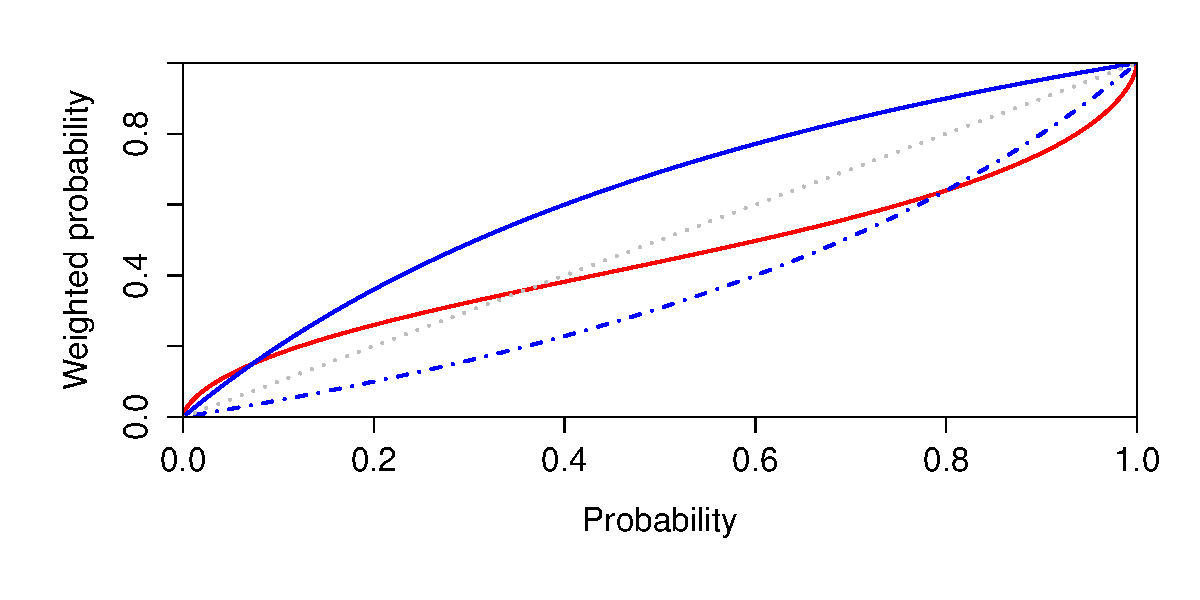
\includegraphics[width = 0.9\textwidth]{decomposition_distortions4}
        \caption{\citet{EbertStrack2015}, online appendix, Figure W1.}
    \end{figure}
\end{frame}





\begin{frame}{Main result}
    \begin{theorem}
        Under Assumptions 1 and 2, for every wealth level there exists an attractive zero-mean binary lottery that is arbitrarily small.
	\end{theorem}

    \begin{corollary}
        Under Assumptions 1 and 2, for every wealth level there exists an attractive, arbitrarily small binary lottery with negative mean.
	\end{corollary}
\end{frame}

\begin{frame}{Main result - interpretation}
    \begin{itemize}
        \item Generally, risk aversion is defined as every fair risk\medskip
        \item Here: skewness preference in the small thus implies that, at every wealth level, a CPT agent is not risk averse.\medskip
        \item Sufficiently small risks are attractive to CPT agents.\medskip
        \item \citet{AzevedoGottlieb2012}: skewness preference in the large, $p\approx 7.2$ for CPT weight $\Rightarrow$ not so small!\medskip
	\end{itemize}
\end{frame}

\begin{frame}{Dynamic consequences}
    \begin{itemize}
        \item What does skewness preference in the small do?\medskip
        \item Consider Markov diffusion $ X= (X_t)_{t \in \mathbb{R}_+ }$
        \[dX_t = \mu(X_t)dt + \sigma (X_t)dW_t\]
        \item Brownian motion $(W_t)_{t \in \mathbb{R}_+ }$, drift $\mu:\mathbb{R} \rightarrow \mathbb{R}$, volatility $\sigma: \mathbb{R}  \rightarrow (0,\infty)$ Lipschitz continuous.\medskip
        \item Investment or gambling strategies: integrable stopping times $\tau$, adapted filtration $(\mathcal{F} _t)_{t \in \mathbb{R}_+ }$\medskip
        \item CPT utility of strategy $\tau$ given $\mathcal{F} _t$, $CPT(X_\tau,\mathcal{F}_t)$\medskip
        \item Hence, we have  time inconsistency \citep{Barberis2012a}: $\tau$ may changed later\medskip
       	\end{itemize}
\end{frame}


\begin{frame}{Dynamic consequences}
    \begin{itemize}
        \item A naive investor does not anticipate that\medskip
        \item He stops at $t$ if $CPT(X_\tau,\mathcal{F}_t) \leq CPT(X_t,\mathcal{F}_t)=U(X_t)$\medskip
        \item $U(X_t) \geq \sup_{\tau \geq t} CPT(X_\tau,\mathcal{F}_t)$
    \end{itemize}
\end{frame}

\begin{frame}{Until the bitter end - CPT agent never stops}
    \begin{theorem}
        \begin{itemize}
        \item Under Assumptions 1 and 2, the naive CPT agent never stops.\medskip
        \item Reference point can be dynamic and change\medskip
        \item Information: simple two-threshold strategy:
        Stoping if utility drop slightly while continuing until utility raises a lot always exceeds stopping.\medskip
	\end{itemize}
\end{theorem}
\end{frame}

\begin{frame}{Where do we stand - summary}
    \begin{itemize}
        \item Cumulative prospect theory generally is one of the most successful alternatives to expected utility theory\medskip
        \item Is one of the standard behavioural approaches\medskip
        \item It is designed for experimental settings\medskip
        \item Extrapolating it to other setting requires care\medskip
        \item It has strong limitations mostly stemming from probability weighting\medskip
    \end{itemize}
\end{frame}




\section{Alternative Theories of Choice under Risk}
\subsection{Reference-Dependent Risk Attitudes}

\frame{\frametitle{Agenda}
\tableofcontents[currentsubsection]
}

\begin{frame}{Limitations of Cumulative Prospect Theory}
 \begin{itemize}
 \item Application of CPT is difficult. Progress in finance and insurance, some micro.\medskip
 \item The exact application drives results, for example, in the disposition effect literature.\medskip
 \item Individual components of CPT are experimentally challenged.\medskip
 \item Probability weighting vs reference dependence.\medskip
 \item Diminishing sensitivity seems largely irrelevant.\medskip
 \end{itemize}
\end{frame}

\begin{frame}{Limitations of Cumulative Prospect Theory}
 \begin{itemize}
 \item Gains and losses are notoriously difficult to identify.\medskip
 \item Interpretation is unclear for normative economics.\medskip
 \item Suppose people follow CPT, and we identify loss aversion and probability weighting.\medskip
 \item Should we then treat their behaviour as a mistake?\medskip
 \end{itemize}
\end{frame}

\begin{frame}{Limitations of Cumulative Prospect Theory}
 \begin{itemize}
 \item How can we address CPT limitations?\medskip
 \item One key issue is the reference point.\medskip
 \item Recent research thinks about explaining its origin and its dynamics.\medskip
     \item \citet{KoeszegiRabin2006, KoeszegiRabin2007} deliver a first attempt based on expectations.\medskip
 \end{itemize}
\end{frame}


\begin{frame}{Reference-Dependent Risk Attitudes}
    \begin{itemize}
         \item \citet{KoeszegiRabin2007} consider an endogenous choice of reference points.\medskip
        \item The reference point has huge impact for economic choices (disposition effect)\medskip
        \item Combine gain/loss utility with standard consumption utility (\citet{Rabin2000}'s critique).\medskip
            \item Allows for stochastic reference points.\medskip
            \item Assume rational decision maker!\medskip
        \end{itemize}
\end{frame}

\begin{frame}{Reference-Dependent Risk Attitudes}
    \begin{itemize}
            \item \citet{KoeszegiRabin2007} distinguish three different cases:\medskip
            \item First, there are small stake gambles that surprise individuals and appear immediately.\medskip
            \item Second, there are small stake gambles that individuals anticipate. Time horizon can be either short or long.\medskip
           \item Third, there are large stage gambles that individual anticipate.\medskip
           \item The context influence the importance of the reference point, how endogenous it is, and the consumption utility.\medskip
                    \end{itemize}
\end{frame}

\begin{frame}{Case 1 - surprise setting}
    \begin{itemize}
        \item Low probability decisions, exogenous expectations.\medskip
        \item Consider lottery: pay \$55 to insure \$100 risk, 50\% probability\medskip
        \item Potential outcomes:\medskip
        \begin{enumerate}[(a)]
            \item status quo reference point: $r = 0$. $\rightarrow$ diminishing sensitivity do not insure\medskip
            \item expect to pay 55: reference point $r = -55$. Lose 45  or gain 55. Loss aversion implies  insurance.\medskip
        \end{enumerate}
        \item Consumption utility is linear. Loss aversion dominates, almost risk-neutral.\medskip
        \end{itemize}
   \end{frame}

 \begin{frame}{Case 2a - short horizon anticipated risks}
    \begin{itemize}
    \item Consider decision shortly before outcome.\medskip
    \item Reference point fixed by past expectations.\medskip
    \item  Fully rational: Expects behaviour only if will to go through with it.\medskip
            \item Define unacclimating personal equilibria (UPE)\medskip
            \item Behaviour where the stochastic outcome generated by utility-maximising choices conditional on expectations equals expectations.\medskip
            \item Follows planned behaviour and selects preferred personal equilibrium (PPE)\medskip
           \item Consumption utility is linear. Strong taste to avoid risk.\medskip
            \end{itemize}
            \end{frame}


     \begin{frame}{Case 2b - long horizon anticipated risks}
    \begin{itemize}
    \item Consider decision long before outcome.\medskip
       \item Committed decision long before outcomes, hence reference point influenced by choice.\medskip
            \item Define choice-acclimating personal equilibria (CPE)\medskip
            \item Individual maximises expected utility given that if determines reference lottery and outcome lottery.\medskip
           \item Consumption utility is linear. Strong taste to avoid risk.\medskip
           \item Key difference: commitment to buy insurance makes decision maker better off.\medskip
    \end{itemize}
\end{frame}

     \begin{frame}{Case 3a - large stake gamble}
    \begin{itemize}
    \item Consider decision long before outcome.\medskip
     \item Consider large gambles,
     \item Consumption utility becomes non-linear and  reference point loses importance.\medskip
     \item Risk aversion reflecting diminishing sensitivity to consumption.\medskip  \end{itemize}
\end{frame}



\begin{frame}{Preference assumptions}
    \begin{itemize}
        \item Wealth $w \in \mathbb{R}$ and reference $r \in \mathbb{R}$ measured by risk-less utility function
               \[u(w | r) = m(w) + \mu ( m(w) - m(r) )^2\]
                \item Reference point is a belief of outcomes, $G$ probability measure
         \[U(w | G)=\int u(w|r)  \,dG(r)\]
        % \item Implies mixed feelings, $50/50$ lottery, outcomes $0/100$, implies 50$:gain to 0, loss to 100.\medskip
        \item Wealth is stochastic: $w$ has measure $F$
        \[U(F|G)=\iint u(w | r) dG(r) dF(w)\]
        \item Abstract from probability weighting for simplicity.\medskip
	\end{itemize}
\end{frame}


\begin{frame}{Assumptions on gain/loss utility}
    \begin{itemize}
        \item A0: $\mu(x) $ continuous, twice differentiable for $x\neq 0$, $\mu(0)=0 $.\medskip
        \item A1: $ \mu(x)$ strictly increasing. \medskip
        \item A2: if $y>x\geq 0 $, then $\mu(y)+\mu(-y) <\mu(x) +\mu(-x) $.\medskip
    \item A3: $ \mu^{\prime\prime}(x) \leq 0 $ for $ x>0$ and $\mu^{\prime\prime}(x) \geq 0$ for $ x<0 $.\medskip
        \item A4: $\frac{\mu^{'}_{-}(0)}{\mu^{'}_{+}(0)} \equiv \lambda >1 $,
    where $ \mu^{\prime}_{+}(0) \equiv \lim_{x \to 0} \mu^{\prime}(\left\lvert x \right \rvert )$ and $ \mu^{\prime}_{-}(0) \equiv \lim_{x \to 0} \mu^{\prime}(-\left\lvert x \right\rvert )$.\medskip
	\end{itemize}
\end{frame}




\begin{frame}{Assumptions on gain/loss utility}
    \begin{itemize}
 	\item A2 and A4 describe loss aversion\medskip
        \item A3 captures diminishing sensitivity\medskip
        \item Sometimes useful: A3$^{\prime}$: $\forall x \neq 0, \mu^{\prime \prime}(x)=0$, i.e., no diminishing sensitivity.\medskip
        \item General assumption: reference point corresponds to expectations.\medskip
        \item Rational expectations, generally people have some idea how they behave and their own environment.\medskip
	\end{itemize}
\end{frame}


\begin{frame}{Risk aversion in surprise situations}
    \begin{itemize}
        \item Suppose $m$ is linear: $m(w)=w$\medskip
        \item The reference point $r$ is fixed\medskip
	\end{itemize}
    \begin{proposition}[1]
        Suppose $m(\cdot)$ is linear and $\mu(\cdot)$ satisfies A3'(no diminishing sensitivity).
        For any lotteries $F,G,H$, and constant $w$,        if $ U(w + F|G) \geq U(w|w)$, then $U(H+F|G) \geq U(H|G)$.\\
    \end{proposition}
\end{frame}

\begin{frame}{Risk aversion in surprise situations}
        \begin{proposition}[1]
        Suppose $m(\cdot)$ is linear and $\mu(\cdot)$ satisfies A3'(no diminishing sensitivity).
        For any lotteries $F,G,H$, and constant $w$, if $ U(w + F|G) \geq U(w|w)$, then $U(H+F|G) \geq U(H|G)$.\\
    \end{proposition}
     \begin{itemize}
        \item If willing to accept $F$ relative to risk-free $r$, positive values of $F$ are gains, negative ones are losses.\medskip
        \item If $F$ is added to lottery $H$ relative to lottery $G$, positive outcomes of $F$ eliminate losses from $H$ relative to $G$, losses from $F$ merely eliminate gains from $H$.\medskip
        \item Hence, individual is more willing to accept $F$.\medskip
        \item If $H=w$ and $G=F$:  less risk averse in eliminating risk that is expected.\medskip
	\end{itemize}
\end{frame}


\begin{frame}{Risk aversion in surprise situations}
    \begin{proposition}[2]
        Suppose $m(\cdot)$ is linear. For any lottery F with positive expected value:
        \begin{enumerate}[(i)]
            \item There exist $A, \varepsilon >0 $ such that if G has $\Pr_G[r \in (k-A, k+A)]< \varepsilon $ for all constants k, then $U(H+F|G)> U(H|G)>U(H-F|G)$ for any lottery H.\medskip
            \item For any continuously distributed lottery G, there is a $\bar{t}>0 $ s.t. for any $t \in (0,\bar{t}]$ and any lottery $H, U(H+t\cdot F|G)> U(H|G)> U(H-t \cdot F|G)$.\medskip
        \end{enumerate}
    \end{proposition}
Identifies attitudes towards $F$ in which the decision maker risk neutral.\medskip
    \begin{enumerate}[(i)]
        \item If sufficiently widely distributed reference lottery, accept F, and reject -F.\medskip
        \item If fixed continuously distributed reference lottery, accept sufficiently small multiple of F, reject the same multiple of -F.\medskip
    \end{enumerate}
Propositions. 1 \& 2 do not imply no risk aversion, just lower risk aversion!
\end{frame}

\begin{frame}{Anticipated risk attitudes}
    \begin{itemize}
        \item Individual now correctly anticipates choice set. \medskip
        \item Cannot commit to choice until shortly before outcome
        \[L=\{D_1,1-q;D_2,q\}, D_1,D_2 \in \bigtriangleup (\mathbb{R})\]
        \item For now, $q=0$, that is, the choice set is certain\medskip
        \item Beliefs are set, reference point exogenous.\medskip
	\end{itemize}
   \end{frame}

\begin{frame}{Anticipated risk attitudes}
     \begin{definition}[UPE]
        A selection $F_1 \in D_1, F_2 \in D_2$ is an unacclimating personal equilibrium (UPE) if for each $l \in 1,2$
        and any $F_l^{\prime} \in D_l$ if
        \[U\left(F_l \mid(1-q) F_1+q F_2\right) \geq U\left(F_l^{\prime} \mid(1-q) F_1+ q F_2\right).\]
    \end{definition}

    \begin{itemize}
    \item  \citet{Koszegi2010}  proves existence.\medskip
        \item  If the person expects to choose $F_1$ and $F_2$ from choice sets $D_1$ and $D_2$, then she expects the distribution of outcomes $(1-q) F_1+q F_2$.\medskip
        \item If this something is the expectation she should be willing to choose  $F_1$ and $F_2$.\medskip
    \end{itemize}
\end{frame}


\begin{frame}{Example}
\begin{itemize}
\item Consider wealth $w$, lottery $L$ with $50/50$ chance of $0,-100$ or pay $-55$.\medskip
\item When is the lottery $L$ a UPE?\medskip
\end{itemize}
\[
\left[\frac{1}{2}(w -100)+\frac{1}{2} w\right]
 +\left[\frac{1}{4} \mu(100)+\frac{1}{4} \mu(-100)\right]
\geq  {[w-55] } + \left[\frac{1}{2} \mu(45)+\frac{1}{2} \mu(-55)\right]
\]
    \begin{itemize}
        \item UPE generally not unique.\medskip
        \item Expectation: plan what to do at the time.\medskip
        \item Idea: select best plan she will follow through on.\medskip
    \end{itemize}
\end{frame}

\begin{frame}{Preferred personal equilibrium }
    \begin{definition}[PPE]
        A selection $F_1 \in D_1, F_2 \in D_2$ is a preferred personal equilibrium(PPE) if it is a UPE,
        and \[U\left((1-q) F_1+q F_2 \mid(1-q) \mathrm{F}_1+qF_2\right) \geq U\left((1-q) \mathrm{F}_1^{\prime}+q \mathrm{~F}_2^{\prime} \mid(1-q) \mathrm{F}_1^{\prime}+q \mathrm{~F}_2^{\prime}\right)\]
        for all $U P E$ selections $F_l^{\prime} \in D_1, F_2^{\prime} \in D_2$.\\
    \end{definition}
\begin{itemize}
\item Choice optimal \alert{conditional on} expectations!
\end{itemize}
\end{frame}

\begin{frame}{Insurance of likely losses}
    \begin{proposition}[3]
    Suppose $m(\cdot)$ is linear. For any $w \in \mathbb{R}$ and mean-zero lottery $F \neq 0$ with bounded support,     there exist $\bar{k}, \bar{t}>0$ such that for any positive $t<\bar{t}, k<\bar{k}$,
    the unique $P P E$ with the choice set $\{w, w+t(F+k)\}$ is to choose w.\\
    \end{proposition}
    \begin{itemize}
        \item Select risk-less $w$ over a sufficiently small, better-than-fair but unattractive bet.\medskip
        \item Loss aversion makes gamble unattractive.\medskip
        \item Key point:  Under CPT, costs correspond to loss in status quo.\medskip
        \item Here: expected costs, such as insurance premium, is a cost, not a loss.\medskip
        \item Reference-dependent utility can explain insurance for likely events that CPT underweights.\medskip
	\end{itemize}
\end{frame}

\begin{frame}{Risk attitudes to expected risk}
    \begin{proposition}[4]
        Suppose $m(\cdot)$ is linear, $\mu(\cdot)$ satisfies A3'.
        If $w+F$ is a PPE in the choice set $\{w, w+F\}$, then for any lottery \[H, U(w+F \mid H)>U(w \mid H)\].\\
    \end{proposition}
    \begin{itemize}
	\item If choice is between risk and insurance, decision maker is at least as risk averse as in  surprise situations.\medskip
	 \item In experiments , people generally are in surprise settings and don't know what comes\medskip
\item Consequently, the experimenter underestimates risk aversion\medskip
\item    Additionally, expecting risk decreases risk aversion.\medskip
    \end{itemize}
\end{frame}

\begin{frame}{Choice-acclimating personal equilibria}

    \begin{definition}[CPE]
        For any choice set $D, F \in D$ is $a$ choice-acclimating personal equilibrium $(C P E)$
        if $U(F \mid F) \geq U\left(F^{\prime} \mid F^{\prime}\right)$ for all $F^{\prime} \in D$.
    \end{definition}\bigskip
     \begin{itemize}
        \item Consider long committed choices\medskip
        \item  Selecting a lottery $F$ determines it as reference point.\medskip
	\end{itemize}
\end{frame}

\begin{frame}{Choice-acclimating personal equilibria}
     \begin{itemize}
           \item Example: lottery $L$ with $50/50$ chance of $(0,-100)$ is a CPE if
  \[
    \left[\frac{1}{2}(w-100)+\frac{1}{2} w\right]
   +\left[\frac{1}{4} \mu(100)+\frac{1}{4} \mu(-100)\right]
     \geq[w-55]+[0] .
\]
        \item UPE: premium 55 can be gain or loss;\medskip
        \item CPE: premium 55 is neither gain nor loss.\medskip
	\end{itemize}
\end{frame}

\begin{frame}{Implications of choice-acclimating personal equilibria}
    \begin{itemize}
        \item Unlike UPE and PPE, for CPE people may want to choose stochastically dominated options\medskip
        \item Idea: give up unlikely gain to avoid losses\medskip
	\end{itemize}
\end{frame}



\begin{frame}{Some discussion}
    \begin{itemize}
        \item Idea of reference-dependent risk attitudes is appealing\medskip
        \item The rationality requirements for the agent are high\medskip
        \item Applications are difficult - the equilibria are challenging to compute in non-trivial settings.\medskip
        \item Not too many applications, room for research, focus more on microeconomics\medskip
	\end{itemize}
\end{frame}



\subsection{Salience Theory}

\frame{\frametitle{Agenda}
\tableofcontents[currentsubsection]
}

\begin{frame}{Salience Theory}
\begin{itemize}
\item Dependent on context, people may be risk averse or risk loving.\medskip
\item People tend to focus on salient aspects in their choices.\medskip
\item Example: Choice between Singapore Airlines and Air Asia.\medskip
\item \citet{BordaloGennaioliShleifer2012, BordaloGennaioliShleifer2013a, BordaloGennaioliShleifer2013b} develop a model of context-dependent choices.\medskip
\item We focus on choices under risk, i.e., \citet{BordaloGennaioliShleifer2012}
\end{itemize}
\end{frame}

\begin{frame}{Salience Theory}
    \begin{itemize}
        \item Key idea: risk preferences not stable but context-dependent.\medskip
        \item \citet{Allais1953} paradox\footnote{See \citet{Allais1979} for translated version.}: irrelevant choice changes risk attitude from risk averse to risk loving.\medskip
        \item Idea: salience/attention to prominent outcomes\medskip
        \item Building blocks:\smallskip
        \begin{itemize}
            \item ordering\medskip
            \item diminishing sensitivity\medskip
            \item salience weighting (\alert{not!} probability weighting)\medskip
        \end{itemize}
	\end{itemize}
\end{frame}

\begin{frame}[t]{Allais paradox}
\begin{itemize}
\item Consider\[L_1(z)=\left\{\begin{array}{lll}\$ 2500 & \text { with prob. } & 0.33\\ \$0 & & 0.01 \\ \$ z & & 0.66\end{array}\right.\]
and
\[L_2(z)=\left\{\begin{array}{lll}\$ 2400 & \text { with prob. } & 0.34 \\ \$ z & & 0.66\end{array}\right.\]\medskip
\end{itemize}
\end{frame}

\begin{frame}[t]{Allais paradox}
\begin{itemize}
\item Consider\[L_1(z)=\left\{\begin{array}{lll}\$ 2500 & \text { with prob. } & 0.33\\ \$0 & & 0.01 \\ \$ z & & 0.66\end{array}\right.\]
and
\[L_2(z)=\left\{\begin{array}{lll}\$ 2400 & \text { with prob. } & 0.34 \\ \$ z & & 0.66\end{array}\right.\]\medskip
\item In experiments: $z=2400$:
\[(2400)= \begin{cases} 2500 \text { with prob. } & 0.33 \\  0 & 0.01 \qquad\prec \qquad L_2(2400)=2400\\  2400 & 0.66\end{cases}
\]
\end{itemize}
\end{frame}

\begin{frame}[t]{Allais paradox}
\begin{itemize}
\item Consider\[L_1(z)=\left\{\begin{array}{lll}\$ 2500 & \text { with prob. } & 0.33\\ \$0 & & 0.01 \\ \$ z & & 0.66\end{array}\right.\]
and
\[L_2(z)=\left\{\begin{array}{lll}\$ 2400 & \text { with prob. } & 0.34 \\ \$ z & & 0.66\end{array}\right.\]\medskip
\item In experiments: $z=0$:
\[L_1(0)= \begin{cases} 2500 \text { with prob. } & 0.33 \\ 0 & 0.67 \end{cases}\qquad \succ \qquad
L_2(0) = \begin{cases} 2400 \text { with prob. } & 0.34 \\ 0 & 0.66\end{cases}\]
\end{itemize}
\end{frame}



\begin{frame}{Cumulative Prospect Theory and Salience}
\begin{itemize}
    \item CPT: in last gamble $w(p=0.01)$ overweighted\medskip
    \item Salience theory: $L_1(2400),L_2(2400) \rightarrow$ 2500 only slightly higher than 2400; 0 a lot lower than 2400.\medskip
    \item Salience theory: $L_1(0),L_2(0) \rightarrow$ outcome zero is standard; 2500 stands out more.\medskip
\end{itemize}
\end{frame}

\begin{frame}{Model of Salience Theory}
    \begin{itemize}
        \item State $s \in S$\medskip
        \item Probability $\pi_s$, such that $\sum_{s \in S} \pi_s=1$\medskip
        \item Choice set $\left\{L_1, L_2\right\}$t\medskip
        \item Payoffs $x_s^i$\medskip
        \item Value function as before, reference-dependent $V$ without decision weights, only local thinking:
        \[    V\left(L_i\right)=\sum_{s \in S} \pi_s v\left(x_s^i\right)\]
     	\end{itemize}
\end{frame}

\begin{frame}{Model of Salience Theory}
    \begin{itemize}
	\item Model features a salience distortion:\medskip
        \item Two steps: salience ranking, then decision weight $\pi_s^i$\medskip
        \item Formally: $x_s=\left(x_s^i\right)_{i=1,2}$, payoffs in state $s$\medskip
        \item $x_s^{-i}$: payoff of lottery $L_j$, $j \neq i$\medskip
        \item $x_s^{\min }, x_s^{\max }$: largest / smallest payoffs in $\mathrm{x}_s$
	\end{itemize}
\end{frame}


\begin{frame}{Salience definition}
    \begin{definition}
        The salience of state $s$ for lottery $L_i, \mathrm{i}=1,2$, is a continuous and bounded function $\sigma\left(x_s^i, x_s^{-i}\right)$ that satisfies three conditions:\\
        \begin{enumerate}
            \item Ordering. If for states $s, \tilde{s} \in S$ we have that $\left[x_s^{\min }, x_s^{\max }\right] \in \left[x_{\tilde{s}}^{\min }, x_{\tilde{s}}^{\max }\right]$, then
    \[
    \sigma\left(x_s^i, x_s^{-i}\right)<\sigma\left(x_{\tilde{s}}^i, x_{\tilde{s}}^{-i}\right) .
    \]
            \item Diminishing sensitivity. If $x_s^j>0$ for $j=1,2$, then for any $\epsilon>0$,
\[
\sigma\left(x_s^i+\epsilon, x_s^{-i}+\epsilon\right)<\sigma\left(x_s^i, x_s^{-i}\right) .
\]
            \item Reflection. For any two states $s, \tilde{s} \in S$ s.t. $x_s^j, x_{\tilde{s}}^j>0, (j=1,2)$, we have
            \[\sigma\left(x_s^i, x_s^{-i}\right)<\sigma\left(x_{\tilde{s}}^i, x_{\tilde{s}}^{-i}\right)\, \text{if and only if}\, \sigma\left(-x_s^i,-x_s^{-i}\right)<\sigma\left(-x_{\tilde{s}}^i,-x_{\tilde{s}}^{-i}\right).\]
        \end{enumerate}
    \end{definition}
\end{frame}

\begin{frame}{Example of Salience computation}
\[
    \sigma\left(x_s^i, x_s^{-i}\right)=\frac{\left|x_s^i-x_s^{-i}\right|}{\left|x_s^i\right|+\left|x_s^{-i}\right|+\theta}, \theta>0
    \]
    \begin{itemize}
        \item ordering: salience rises if distance of  $x_s^i$ and $x_s^{-i}$ rises\medskip
        \item diminishing sensitivity: as average payoff gets farther from zero, salience reduces $\left|x_s^1\right|+\left|x_s^2\right|$\medskip
        \item reflection: salience is shaped by the magnitude, not sign\medskip
        \item (example: symmetric additional dropped for $N>2$)\medskip
        \item Results mostly driven by ordering and diminishing sensitivity.\medskip
	\end{itemize}
\end{frame}

\begin{frame}{Ordering}
\begin{figure}
\centering
    \includegraphics[width = 0.99\textwidth]{ordering}
    \caption{\citet{BordaloGennaioliShleifer2012}, Figure 1a.}
    \end{figure}
\end{frame}

\begin{frame}{Diminishing sensitivity}
\begin{figure}
\centering
    \includegraphics[width = 0.99\textwidth]{diminishing_sensitivity}
    \caption{\citet{BordaloGennaioliShleifer2012}, Figure 1b.}
    \end{figure}
\end{frame}


\begin{frame}{Reflection}
\begin{figure}
\centering
    \includegraphics[width = 0.99\textwidth]{reflection}
    \caption{\citet{BordaloGennaioliShleifer2012}, Figure 1c.}
    \end{figure}
\end{frame}

\begin{frame}{Salience measure}
    \begin{definition}
        Given states $s, \tilde{s} \in S$, we say that for lottery $L_i \mathrm{~s}$ $s$ is more salient than $\tilde{s}$ if $\sigma\left(x_s^i, x_s^{-i}\right)>\sigma\left(x_{\tilde{s}}^i, x_{\tilde{s}}^{-i}\right)$.
        Let $k_s^i \in\{1, \ldots,|S|\}$ be the salience ranking of state $s$ for $L_i$, with lower $k_s^i$ indicating higher salience.
        All states with the same salience obtain the same ranking(no jumps). Then the local thinker transforms the odds $\frac{\pi_{\tilde{s}}}{\pi_s}$ of $\tilde{s}$ relative to $s$ into the odds $\frac{\pi_s^i}{\pi_s^i}$, given by:
        \[
        \frac{\pi_{\tilde{s}}^i}{\pi_s^i}=\delta^{k_{\tilde{s}}^i-k_s^i} \cdot \frac{\pi_{\tilde{s}}}{\pi_s}, \text{\quad where } \delta \in(0,1]
        \]
        By normalising $\sum_s \pi_s^i=1$ and defining $\omega_s^i=\frac{\delta^{k_s^i}}{\left(\sum_r \delta^{k_r^i} \cdot \pi_r\right)}$, the decision weight is: $\pi_s^i=\pi_s \cdot \omega_s^i$
        $\Rightarrow$ local thinker overweights most salient states.
    \end{definition}
\end{frame}

\begin{frame}{Model}
    \begin{itemize}
        \item $\delta=1 \Rightarrow$ standard model, $\omega_s^i=1$\medskip
        \item $\delta<1 \Rightarrow$ local thinker\medskip
        \item state $s$ is overweighted, if $\left(\omega_s^i>1\right.$, or $\left.\delta^{k_s^i}>\sum_r \delta_r^{k_r^i} \cdot \pi_r\right)$\medskip
        \item $\delta \rightarrow 0$: decision based on most salient state\medskip
        \item $\delta$ is independent of objective state probabilities!\medskip
    \end{itemize}
\end{frame}

\begin{frame}{Some remarks}
    \begin{itemize}
        \item weighting depends on salience, not low probability\medskip
        \item low-probability can be most overweighted, but also underweighted\medskip
        \item choice of state space / alternative lottery unclear\medskip
        \item some cases: no alternative $\Rightarrow$ take zero? Open question\medskip
    \end{itemize}
\end{frame}

\begin{frame}{Risk attitudes}
        \begin{itemize}
            \item Suppose linear value function\medskip
            \item Compare sure prospect: $L_0=(x,1)$ and mean preserving spread \[L_1=\left(x+g, \pi_g ; x-l, 1-\pi_g\right)\] with $g \pi_g=\left(1-\pi_g\right) l$ and $x, g, x-l >0$\medskip
            \item Two states $s_g = (x + g, x)$ and  $s_l=(x-l, x)$\medskip
            \item Local thinking value function \[V^{LT}(L)=\sum_{s \in S} \pi^i_s v\left(x_s^i\right)=\sum_{s \in S} \pi_s \omega ^i_s v\left(x_s^i\right)\]\medskip
        \end{itemize}
    \end{frame}

\begin{frame}{Risk attitudes}
    \begin{itemize}
        \item $\delta<1 \Rightarrow$ prefer $L_1$ if $s_g$ more salient, $\sigma(x+g, x)>\sigma(x-l, x)$\medskip
        \item  Using $g \pi_g=\left(1-\pi_g\right) l$, consider \[\sigma\left(x+\frac{1-\pi_g}{\pi_g} \cdot l, x\right)>\sigma(x-l, x)\]
        \item Above holds if $\pi_g \simeq 0$ (gain unlikely) because $g$ is high $\Rightarrow$ risk taking\medskip
        \item Diminishing sensitivity: if $g=l, x-l<g+x$ implies that the loss is salient,$\pi_g=\frac{1}{2} \Rightarrow$ risk averse\medskip
        \item $\Rightarrow \pi^*_g <\frac{1}{2}$, below risk seeking, above averting\medskip
    \end{itemize}
\end{frame}


\begin{frame}{Context-Dependent Probability Weighting Function}
\begin{figure}
\centering
    \includegraphics[width = 0.5\textwidth]{context_dependent_weighting}
    \caption{\citet{BordaloGennaioliShleifer2012}, Figure 2.}
    \end{figure}
\end{frame}


\begin{frame}{Risk attitudes}
    \begin{definition}
        A salience function is convex if, for any state with positive payoffs $(y, z)$ and any $x, \epsilon>0$, the difference $\sigma(y+x$, $z+x)-\sigma(y+x+\epsilon, z+x+\epsilon)$ is a decreasing function of the payoff level $x$ (concave if increasing in $x$).
    \end{definition}
    \begin{Lemma}
        If the salience function is convex, then $r=v^{L T}\left(L_0\right)-$ $v^{L T}\left(L_1\right)$ weakly decreases with $x$   (concave if increases with $x$).
    \end{Lemma}
   \begin{itemize}
   \item If diminishing sensitivity weakens with $x$, a higher payoff level raises the relative attractiveness of  $L_1$.\medskip
   \item If $\pi_g^* $ increases, it raises risk seeking
    \end{itemize}
\end{frame}

\begin{frame}{Some critical remarks}
    \begin{itemize}
        \item \citet{Kontek2016}: Certainty Equivalent not necessarily defined\medskip
        \item Monotonicity for $N>2$ violated\medskip
        \item Mixed experimental evidence if estimated from indifference curves\medskip
	\item \citet{Dertwinkel-KaltFrey2023} find experimental support for a theory of optimal stopping under salience theory.\medskip
        \item Some strong empirical support by \citet{CosemansFrehen2021}\medskip
        \item There is room for research\medskip
	\end{itemize}
\end{frame}

\begin{frame}{Summary and Outlook}
\begin{itemize}
\item Descriptive theories of choice under risk: Cumulative Prospect Theory\medskip
\item Popular approach but challenging to apply\medskip
\item Severe issues arising from probability weighting\medskip
\item There are alternatives developed since 2006 but not much explored in finance\medskip
\item Dynamic theories even less so\medskip
\end{itemize}
\end{frame}

\begin{frame}[allowframebreaks]
    \frametitle{References}
    \renewcommand{\bibfont}{\normalfont\footnotesize}
    \printbibliography
\end{frame}

\end{document}
